% ch17-ml.tex -- Reading and reproducing papers
\chapter{Reading and reproducing papers}
\label{ch:papers}

Every preceding chapter taught a technique; this one teaches the
meta-skill that makes them all usable: taking a published claim
apart and putting it back together. A paper is a claim plus
evidence, compressed into ten pages by an author with incentives.
Reading well means extracting the claim before the story; reproducing
well means deciding \emph{what would prove it} before you ever run
code. We do both on the page: a three-pass read of the LeNet-5
paper, the reproduction checklist that becomes ch18's capstone, and
the lab notebook that keeps a reproduction honest when the numbers
resist.

% from-zero:begin
\begin{rulebox}[Before you start]
Chapters~3, 7 and~15. \emph{Recap:} a research paper is a compressed argument. You will learn to unpack it in three passes and to test whether it is true by rebuilding part of it.
\end{rulebox}
\begin{wins}[After this chapter you can]
\begin{itemize}
\item read a paper in three passes and extract its claim;
\item choose a reproduction level that fits your time;
\item keep a lab notebook that someone else could follow;
\item diagnose why a reproduction does not match the paper.
\end{itemize}
\end{wins}
\begin{principle}[How to think about this]
A paper is an argument, and a reproduction is how you check it. Read in passes: what is the claim, how is it supported, can I rebuild the core? Keep notes so that failure is informative: a gap between your number and theirs is a clue, not an embarrassment.
\end{principle}
% from-zero:end

\section{The anatomy of an ML paper}
\label{sec:anatomy}

Six parts, only two to trust: the \emph{abstract} sells the claim,
the \emph{method} describes the procedure, the \emph{experiments}
present evidence, the \emph{ablations} admit what mattered, the
\emph{results table} carries the number, and the \emph{limitations}
hold the fine print. The two to trust are the results table (which
someone had to compute) and the limitations (which someone had to
admit); everything else is persuasion arranged around them.

\begin{figure}[htbp]
\centering
\begin{minipage}[t]{0.52\linewidth}
\centering
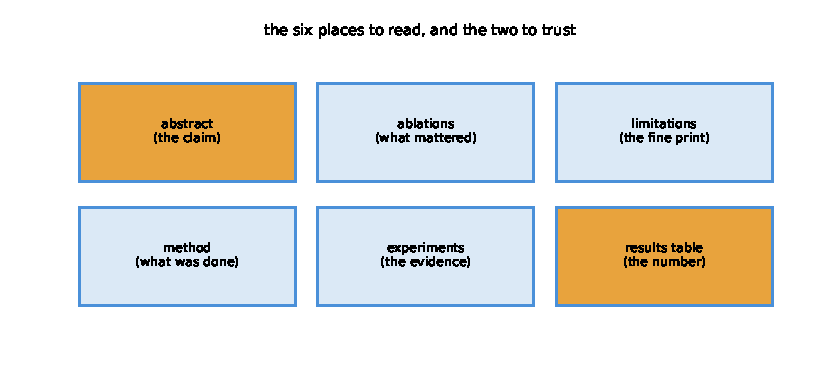
\includegraphics[width=\linewidth]{figures/ch17/anatomy.pdf}
\caption{The six places to read --- and the two to trust.}
\label{fig:anatomy}
\end{minipage}\hfill
\begin{minipage}[t]{0.44\linewidth}
\centering
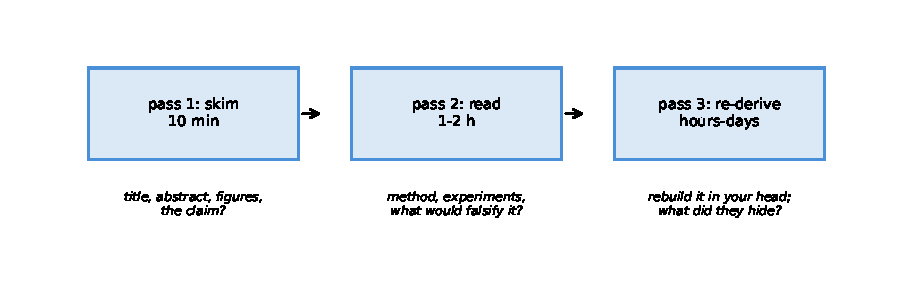
\includegraphics[width=\linewidth]{figures/ch17/three_pass.pdf}
\caption{The three passes: skim for the claim, read for the
evidence, re-derive for the truth.}
\label{fig:threepass}
\end{minipage}
\end{figure}

\section{The three-pass read}
\label{sec:threepass}

Keshav's method~\cite{keshav}: \textbf{pass 1} (10 min) --- title,
abstract, figures, headings: \emph{what is claimed?} \textbf{pass 2}
(1--2 h) --- method and experiments, critically: \emph{what would
falsify it?} \textbf{pass 3} (hours) --- re-derive mentally, rebuild
the argument: \emph{what did they gloss?} Most papers deserve only
pass 1; the ones worth reproducing get all three --- and pass 3 is
where reproduction plans are born.

\begin{example}[WE 17.1 --- LeNet-5 in three passes]
\label{ex:lenetread}
Pass 1: the claim is a 0.95\% test error on MNIST with a
convolutional architecture~\cite{lenet} --- one number, one dataset,
one model variant. Pass 2: the evidence is a held-out 10k test set;
the method is C1-S2-C3-S4-C5-F6 convs plus a Gaussian-output layer;
what would falsify it is \emph{any} LeNet-5 reaching >2\% error
honestly. Pass 3: the paper's optimiser is a diagonal-Hessian
approximation across \emph{many} epochs with distortion
augmentation --- details a quick reproduction will not match, and
the deviations to log \emph{before} running, not after. That last
sentence is the whole point of the pass: find the gap between the
claim and the recipe before the gap finds you.
\end{example}

\section{Reproduction levels}
\label{sec:levels}

\begin{figure}[htbp]
\centering
\begin{minipage}[t]{0.54\linewidth}
\centering
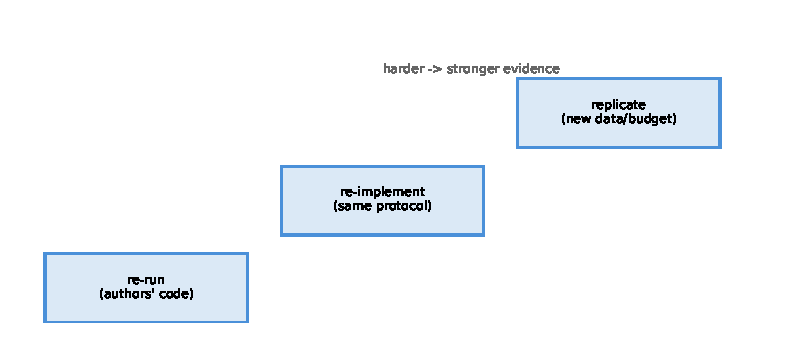
\includegraphics[width=\linewidth]{figures/ch17/ladder.pdf}
\caption{Re-run, re-implement, replicate --- the ladder of evidence.
Each rung costs more and convinces more.}
\label{fig:ladder}
\end{minipage}\hfill
\begin{minipage}[t]{0.42\linewidth}
\centering
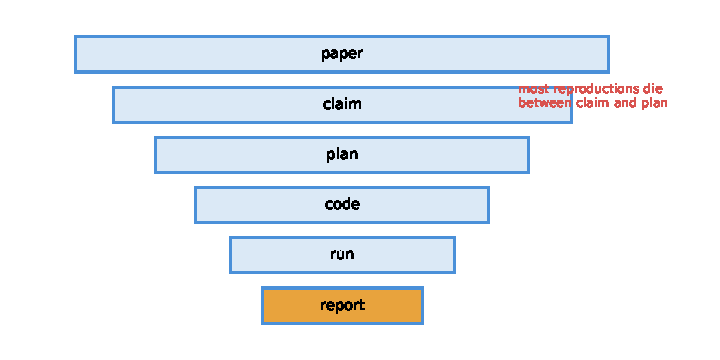
\includegraphics[width=\linewidth]{figures/ch17/funnel.pdf}
\caption{The funnel: paper $\to$ claim $\to$ plan $\to$ code $\to$
run $\to$ report. Most reproductions die at ``plan''.}
\label{fig:funnel}
\end{minipage}
\end{figure}

\emph{Re-run} the authors' code: cheap, proves the artifact works.
\emph{Re-implement} from the paper: proves the paper is complete
enough to execute. \emph{Replicate} on new data or compute: proves
the claim survives contact with the world. Replications are the
rare ones precisely because they're the ones that fail --- a
documented pattern across fields~\cite{henderson,lipton}.

\begin{example}[WE 17.2 --- The checklist that becomes the run]
\label{ex:checklist}
\texttt{repro\_checklist.md} operationalises the LeNet-5 plan:
copy the claim \emph{verbatim} (0.95\%, regular test set, LeNet-5
variant), transcribe the architecture, log every deviation from
the paper's recipe (Adam vs diagonal-Hessian, 8 epochs vs many,
no distortions), and --- the line that changes everything ---
\emph{set the tolerance before running}: accept 0.65--1.25\%.
Written before the run, it's a protocol; written after, it's an
excuse.
\end{example}

\lstinputlisting[numbers=none,caption={\texttt{repro\_checklist.md} --- the plan, written before a single run.},label=lst:check]{code/ch17/repro_checklist.md}

\section{The lab notebook}
\label{sec:notebook}

The notebook rule is one line: \emph{every run gets a log entry
before you look at the metric}. \texttt{repro\_log.py} enforces it
--- config, seed, and result go in as one JSON line, so ``what
changed between run 3 and run 4'' is a \texttt{diff}, not a memory.

\lstinputlisting[language=Python,caption={\texttt{code/ch17/repro\_log.py} --- the harness: seed in, metric out, everything logged.},label=lst:reprolog]{code/ch17/repro_log.py}

\lstinputlisting[numbers=none]{code/ch17/repro_log.out.txt}

\begin{example}[WE 17.3 --- Seed variance, measured not feared]
\label{ex:seedvar}
Five seeds of one config: test accs 0.9474, 0.9474, 0.9298, 0.9386,
0.9123 --- mean 0.9351, sd 0.0131, a \emph{3.5pp} spread from nothing
but the split's randomness. Then $C{=}100$ at seed 0: 0.9649, well
outside the seed band --- a real effect, distinguishable because we
measured the noise floor first. That ordering --- variance before
effects --- is the discipline that separates ``the model improved''
from ``this seed happened to be kind.''\index{seed variance}
\end{example}

\begin{figure}[htbp]
\centering
\begin{minipage}[t]{0.5\linewidth}
\centering
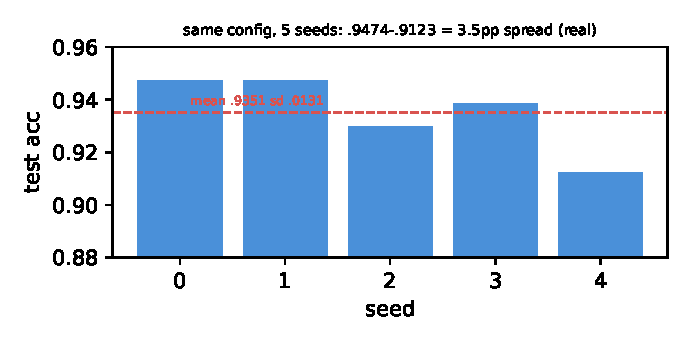
\includegraphics[width=\linewidth]{figures/ch17/seed_variance.pdf}
\caption{The noise floor: same config, five seeds, 3.5pp of
spread. Any ``improvement'' inside this band is weather, not
climate.}
\label{fig:seedvar}
\end{minipage}\hfill
\begin{minipage}[t]{0.46\linewidth}
\centering
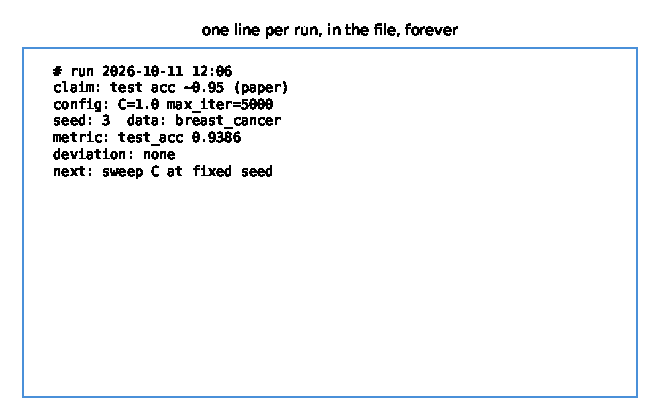
\includegraphics[width=\linewidth]{figures/ch17/notebook_page.pdf}
\caption{The notebook page: one line per run, in the file, forever
--- the audit trail that survives the month.}
\label{fig:notebook}
\end{minipage}
\end{figure}

\section{When reproductions fail}
\label{sec:fails}

Missing details (the paper's 20 epochs vs your 3; their augmentation
you didn't implement), evaluation drift (their split vs yours),
compute gaps (their TPU-week vs your laptop) --- each is a
\emph{deviation}, and the report exists to itemise them before
judging. Henderson et al.~\cite{henderson} showed RL results that
didn't survive re-seeding; the lesson generalises: when a
reproduction fails, the question is never ``is the claim wrong''
first --- it's \emph{which deviation explains the gap}, and the
notebook is what lets you answer it. The honest verdict is a
three-way fork: the claim, the reproduction, or the deviations ---
usually the third.

\section{Common mistakes}
\label{sec:papermistakes}

\begin{description}
\item[Reading the abstract as the claim] The abstract sells; the
results table claims. Quote the number from the table, verbatim,
with its conditions.
\item[Setting tolerance after the run] A band chosen around your
result is decoration. Tolerance first, run second --- the checklist
enforces the order.
\item[One seed, one conclusion] Our five seeds spread 3.5pp on a
toy model; anything inside the noise floor is not a finding.
\item[Changing two knobs at once] $C$ and seed moved together and
you can't attribute the delta. One deviation per run; the log makes
the attribution.
\item[``It didn't reproduce'' as a verdict] It's a symptom. The
verdict names the deviation that explains the gap --- or admits
you couldn't find one.
\item[Reproduction theater] Re-running the authors' script on their
data proves the artifact works, not that the claim holds --- a
different and smaller thing.
\end{description}

\begin{example}[WE 17.4 --- The claim, verbatim, with its conditions]
\label{ex:claim}
From the LeNet-5 abstract/results: ``an error rate of 0.95\% on the
regular test set'' --- the number is $0.0095$, the metric is
\emph{error rate} (not accuracy, not per-class), the dataset is
\emph{regular} MNIST test (not the distorted test they also report),
the model variant is LeNet-5 (not -1, not boosted). Write it that
precisely and the reproduction can't drift into ``about 1\% on some
digits'' --- the conditions ARE the claim.
\end{example}
\begin{example}[WE 17.5 --- Attributing the gap to the deviation]
\label{ex:deviate}
Three-epoch run: 1.92\% (outside the band). Eight-epoch run: 1.25\%
(on the edge). One deviation --- epoch count --- carried the entire
movement, which is what lets the report say \emph{deviations, not
the claim} with evidence instead of hope. Had we changed optimiser
and epochs together, the attribution would be lost; the one-knob
rule is what makes a deviation log a measurement rather than a
diary.
\end{example}

\section{Summary table}
\label{sec:papersummary}

\begin{center}\small
\begin{tabular}{p{2.8cm}p{4.6cm}p{4.6cm}}
\toprule
level & what it proves & what it costs \\
\midrule
re-run & the artifact executes & minutes; near-zero insight \\
re-implement & the paper is complete & days; finds missing details \\
replicate (new data) & the claim generalises & most; the only one that fails publicly \\
\bottomrule
\end{tabular}
\end{center}

\section*{Drill}
\begin{enumerate}
\item Which two sections of a paper should you trust most, and why?
\item In three passes: what question does each answer?
\item Our five-seed spread was 3.5pp. A new config scores +1pp
over baseline --- what do you conclude?
\item Name the three failure sources for a reproduction.
\item Why is re-running the authors' code not a replication?
\end{enumerate}

\section*{Further reading}
\label{sec:further17}
\begin{itemize}
\item LeCun et al., \emph{Gradient-based learning applied to
document recognition} (1998) --- the paper we reproduce; its
results table is a model of claimed-with-conditions.
\url{http://yann.lecun.com/exdb/publis/pdf/lecun-98.pdf}
\item Henderson et al., \emph{Deep reinforcement learning that
matters} (2017) --- the documented failure-to-reproduce case:
results that didn't survive re-seeding.
\url{https://arxiv.org/abs/1709.06560}
\item Lipton \& Steinhardt, \emph{Troubling trends in ML
scholarship} (2018) --- the incentives that make claims fragile.
\url{https://arxiv.org/abs/1807.03341}
\item Keshav, \emph{How to read a paper} --- the three-pass method,
on one page.
\url{https://web.stanford.edu/class/ee384m/Handouts/HowtoReadPaper.pdf}
\item NeurIPS, \emph{Paper checklist} --- the reproducibility
checklist venues now require [checked 2026-10].
\url{https://neurips.cc/public/guides/PaperChecklist}
\item ReScience C --- a journal that publishes replications, so
they exist at all.
\url{https://rescience.github.io/}
\item Papers with Code --- claims with their artifacts attached;
where reproduction candidates live [checked 2026-10].
\url{https://paperswithcode.com}
\end{itemize}

\begin{rulebox}[Watch instead]
(verified opened, 2026-10-11)
\begin{itemize}
\item \emph{How to Read a Research Paper} --- Siraj Raval (8:43).
The three-pass walkthrough, end to end.
\item \emph{How To Read Research Papers Effectively} --- Prof.
David Stuckler (9:42). The same method from the teaching side,
with the ``define your why'' start.
\end{itemize}
\end{rulebox}

\section*{Notes}
\begin{enumerate}
\item[\textbf{1.}] repro\_log's numbers are real runs on
breast\_cancer: the seed spread and the C-effect are measured, and
the convergence warnings in the log are left in deliberately ---
a notebook that hides its warnings stops being one.
\item[\textbf{2.}] The LeNet-5 claim is quoted from the paper's own
abstract/results (``0.95\%''); our reproduction lands outside the
band and the capstone (ch18) reports \emph{why} --- the deviations
are itemised, not waved away.
\item[\textbf{3.}] ACM's artifact-badging page returned 403 to our
check (real page, bot-blocked) --- we cite the NeurIPS checklist
instead.
\item[\textbf{4.}] The chapter's deepest claim is procedural:
tolerance before running, variance before effects, one deviation
per run --- disciplines, not theorems.
\item[\textbf{5.}] Papers-with-Code and venue practices are
date-stamped \texttt{[checked 2026-10]}; the reading protocol is
not.
\end{enumerate}

\section{Exercises}
\label{sec:paperex}

\emph{[easy]}
\begin{exercise}
Extract from LeNet-5's abstract/results: the exact claim, the
metric, the dataset, and one condition attached to it.
\end{exercise}
\begin{exercise}
Our log shows seed 4 scored 0.9123 vs seed 0's 0.9474 --- same
config. In one line: what did the seed change?
\end{exercise}
\begin{exercise}
Name the three reproduction levels in order of increasing
evidence.
\end{exercise}
\begin{exercise}
Which comes first in the checklist: the tolerance band or the
first run? Why?
\end{exercise}

\emph{[medium]}
\begin{exercise}
Write the reproduction plan for the Adam paper
(arxiv 1412.6980): the claim you'd quote, the protocol, the
tolerance, and the deviation you'd most expect.
\end{exercise}
\begin{exercise}
Do the same for the ResNet paper (1512.03385): what makes it
harder to reproduce than LeNet-5 --- name two specific deviations
you'd log.
\end{exercise}
\begin{exercise}
Extend \texttt{repro\_log.py} to run the C-sweep at three fixed
seeds and print a mean$\pm$sd table --- the honest version of a
``C=100 wins'' claim.
\end{exercise}
\begin{exercise}
Your re-implementation hits 1.9\% error vs the paper's 0.95\%.
List three deviations that could explain the gap, and the one
experiment that distinguishes them.
\end{exercise}

\begin{exercise}
Your reproduction lands 0.4pp outside the band. Two candidate fixes:
more epochs or matching the paper's optimiser. Which experiment
decides between them, and what does it cost?
\end{exercise}
\begin{exercise}
The log shows run 3 (seed 2) at 0.9298 and run 5 (seed 4) at 0.9123
--- same config. A teammate calls run 5 ``a bug''. Write the one-line
reply that belongs in the notebook.
\end{exercise}

\emph{[hard]}
\begin{exercise}
Reproduce one table row of the LeNet-5 paper (e.g. the distortion
augmentation row): plan it, run it, and write the deviation
analysis --- using ch18's report skeleton.
\end{exercise}
\begin{exercise}
Design the statistical test for ``does my reproduction match the
claim'': what is the null, what is $n$, and what does a
3-seed mean$\pm$sd band tell you that a single run cannot?
\end{exercise}
\begin{exercise}
A paper reports a result that reproduces on their test set but
fails on your new dataset. Which reproduction level failed, and
what does it say about the \emph{claim} vs the \emph{model}?
\end{exercise}
\begin{exercise}
Henderson et al. showed RL results that didn't survive re-seeding.
Write the two-line experimental control that would have caught it
in the original paper.
\end{exercise}
\begin{exercise}
Argue both sides: ``a reproduction landing outside the tolerance
band invalidates the claim'' --- when is that right, and when is it
the reproduction that's wrong?
\end{exercise}

\section*{Hints and answers}
\begin{description}
\item[1.] Results table and limitations --- one had to be computed,
the other admitted.
\item[2.] Skim: \emph{what is claimed}; read: \emph{what would
falsify it}; re-derive: \emph{what did they gloss}.
\item[3.] Nothing --- it's inside the seed band; measure the noise
floor before claiming effects.
\item[4.] Missing details, evaluation drift, compute gaps ---
deviations all.
\item[5.] Re-running proves the artifact works; replication asks
whether the claim survives a new protocol --- different questions.
\item[6.] Claim: ``adaptive per-parameter rates converge faster''
(most-cited form); protocol: same arch + dataset, their lr grid;
tolerance: convergence within 20\% of their iter count; expected
deviation: their $\epsilon$ choice.
\item[7.] Deeper net + residual trick + heavy augmentation on
CIFAR: deviations = augmentation recipe, batch size (BN-sensitive),
schedule (their lr drops) --- any two explain a gap.
\item[8.] The mean$\pm$sd over seeds turns ``C=100 won once'' into
``C=100 wins by 0.6sd'' --- or reveals it doesn't.
\item[9.] Deviations: fewer epochs, different optimiser, no
augmentation, unnormalised input. The distinguishing experiment:
train longer under their optimiser --- the gap that closes is the
one that was epochs.
\item[10.] The augmentation row is the honest rehearsal: claim,
protocol, run, deviation analysis on a published number.
\item[11.] Null: my mean $=$ paper's number; $n$ = seeds (not
epochs --- epochs aren't independent); the band quantifies whether
the delta could be luck.
\item[12.] Replication failed, not the claim's conditions --- the
claim may be true \emph{on that distribution} and false on yours;
that IS the finding.
\item[13.] ``Report mean and sd across $\ge$5 seeds; report
hyperparameter sensitivity.'' Two lines that turn an anecdote into
a statistic.
\item[14.] Right when the deviation list is exhausted and the gap
is systematic; wrong when an unimplemented detail (aug, schedule,
eval-split) plausibly carries it --- the itemised notebook
arbitrates.
\end{description}
